\documentclass[10 pt]{book}


\usepackage[utf8]{inputenc} % Input encoder, basically for English
\usepackage[table]{xcolor} % Color your document
\usepackage[skins]{tcolorbox} % Colored / nice textbox
\usepackage[document]{ragged2e}
\usepackage[short, nodayofweek, level, 12hr]{datetime}
\usepackage[usestackEOL]{stackengine}

\usepackage{multicol} % Distribute paragraph in muticolumn
\columnseprule = 0.5 mm % Column separator rule width

\usepackage
{
 array, % Manipulate the table rules
 listings, % Code listing
 graphicx, % Picture add and design with graphics
 authblk, % Author affiliation
 tikz, % Graphical plot
 pgfplots, % Graph plots
 tabularx, % More flexible formatted table
 lipsum,
 mVersion, % Adding version later of date
 framed, % For make a frame to CodeListing or any place.
 longtable, % Create and break out large / long table
 wrapfig, % Wrap the figure with text
}

\usepackage[hidelinks]{hyperref} % Add hyperlink / clickable link


\setVersion{0.0}
\increaseBuild % Will update version at each recompilation


\title{Programming Document}
\author
{
	Sofiullah Iqbal Kiron\\
	\href{mailto:sofiul.k.1023@gmail.com}{sofiul.k.1023@gmail.com}
}
\date{11 April, 2020 \\ \currenttime \\ Version: \version}
\affil{BSMRSTU, Department of CSE \\ SHIICT}


\lstset
{
 language = C++,
 backgroundcolor = \color{black!5},
 basicstyle = \footnotesize\ttfamily,
 keywordstyle = \color{blue},
 commentstyle = \color{green!80},
 showstringspaces = false,
 stringstyle = \color{red},
 captionpos = b
}


\hypersetup
{
	colorlinks = true,
	linkcolor = violet,
	filecolor = magenta,
	urlcolor = cyan,
	pdftitle = {Wanna be a programmer?},
	bookmarks = true,
	hyperindex = true, % Makes the page numbers of index entries into hyperlinks
	linktocpage = false, % Makes the page numbers instead of the text to be link in the Table of Contents
	breaklinks = false, % Allows links to be broken into multiple lines
	frenchlinks = false, % Use small caps instead of colours for links
}


\renewcommand\contentsname{A-Z Menu}
\renewcommand\chaptername{Unit}


\begin{document}


\pagecolor{green!90}
\maketitle
\pagecolor{white}
\tableofcontents
\listoffigures
\listoftables

{
	\raggedleft\vfill\itshape\Longstack[l] %You can change this properties to add more formation. As, \Longstack[l], \hfill, \raggedright, not \itshape, etc.
		{
			Thank You,\\
			Sofiullaha Iqbal Kiron.
		}\par
}

\chapter{Quotes}
\begin{flushleft}
	\begin{tcolorbox}[arc=3mm, width=6.8 cm, colback=red!5!white, colframe=red!75!black]
		Examples are better than $1000$ words.
	\end{tcolorbox}
\end{flushleft}

\begin{flushright}
	\begin{tcolorbox}[enhanced, title=Steve Jobs, attach boxed title to bottom right, boxed title style={arc=3mm, colframe=green}, drop large lifted shadow=blue!70, sharp corners]
		Everybody should learn how to program a computer because it teaches how to \textcolor{blue}{THINK}.
	\end{tcolorbox}
\end{flushright}

\begin{tcolorbox}[title=Winner, after title={\hfill\colorbox{blue}{Muhammad Ali}},
colback=red!5!white,colframe=red!75!black,fonttitle=\bfseries, sharp corners]
	I hated every minute of training. But I said, "don't quit, suffer now and live the rest of your life as a champion."
\end{tcolorbox}

\tcbset{frogbox/.style={enhanced,colback=green!10,colframe=green!65!black,
enlarge top by=5.5mm,
overlay={\foreach \x in {2cm, 3.5cm} {
\begin{scope}[shift={([xshift=\x]frame.north west)}]
\path[draw=green!65!black,fill=green!10,line width=1mm] (0,0) arc (0:180:5mm);
\path[fill=black] (-0.2,0) arc (0:180:1mm);
\end{scope}}}}}
\begin{flushright}
\begin{tcolorbox}[frogbox, arc=3 mm, width=4 cm]
You lost?
\end{tcolorbox}
\end{flushright}

\begin{tcolorbox}[width=7cm]
	Just practice and keep learning...
\end{tcolorbox}

\begin{flushright}
	\begin{tcolorbox}[title={Juma Ikangaa, marathoner}, colback=red!5!white, colframe=red!75!black, fonttitle=\bfseries]
		The will to win means nothing without the will to prepare.
	\end{tcolorbox}
\end{flushright}

%Chapter 2.
\chapter{C++, Problems and Algorithm}
\section{Evolution of C}
\begin{figure}[hbtp]
\centering
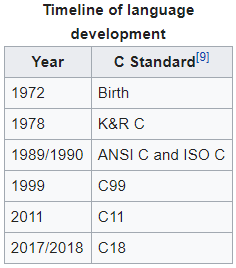
\includegraphics[width=200 px]{Timeline of C language.png}
\caption{Evolution Graph of C}
\end{figure}
C supports variable sized arrays from C99 standard.

\section{Array}
Here we will discuss about array data structure.\\
Reference: \href{https://www.geeksforgeeks.org/array-data-structure/}{GfG}\\

\subsection{Array rotation}
\subsection{Making subarray}
A subarray is a contiguous part of an array. An generated array that are already part of an another array.\\
e.g. : A given array - {1, 2, 3, 4}\\
Subarray of this array:
{1}, {2}, {3}, {4}, {1, 2}, {2, 3}, {3, 4}, {1, 2, 3}, {2, 3, 4}, {1, 2, 3, 4}
Given arrays are subarray of given array. A array holds $\frac{n(n+1)}{2}$ subarrays where $n$ is the number of elements in main array.

\section{Memory Allocation}
\subsection{Memory Layout of C}
Typical memory layout of C consists with following segments:-
\begin{enumerate}
	\item Text segment
	\item Initialized data segment
	\item Uninitialized data segment
	\item Stack
	\item Heap
\end{enumerate}
For better understanding, look at the block diagram below:-\\
\begin{figure}
	\centering
	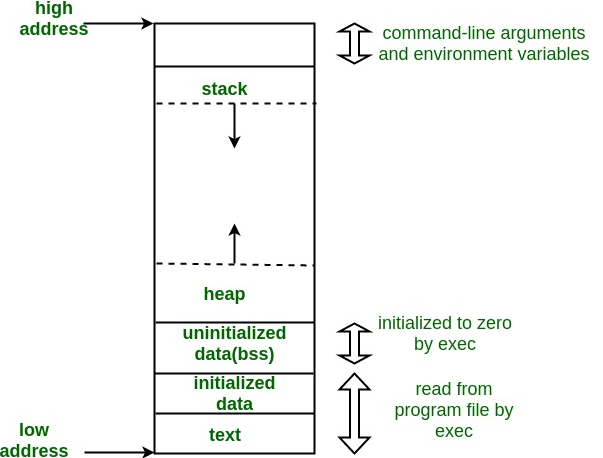
\includegraphics[width=200px, height=140px]{C memory layout, GfG.png}
	\caption{C memory layout, GfG}
\end{figure}
\pagebreak

\textbf{Short explanation:}
\begin{itemize}
	\item[$\rightarrow$] \textbf{A text segment}, known as code segment or simply text holder, is one of the section of a program that contains executable instructions as a text. As a memory region, a text segment may be placed below the heap or stack in order to prevent heaps and stack overflows from overwriting it.
	\item[$\rightarrow$] \textbf{Initialized data segment} usually called \textbf{Data Segment (\textcolor{red}{DS}}), is a portion of virtual address space of a program, which contains \textit{global variables} and \textit{static variables} that are initialized by the programmer.
	\item[$\rightarrow$] \textbf{Uninitialized data segment}, generally known as \textbf{\textcolor{red}{BSS}}, named after an ancient assembler operator that stood for "\textit{block started by symbol}". It contains all global variables and static variables that are initialized to zero or do not have explicit initialization in source code.
	\item[$\rightarrow$] \textbf{Stack} is the segment for storing non-static and local variables.
	\item[$\rightarrow$] \textbf{Heap} is the segment where dynamic memory allocation usually takes place. The heap area began at the end of the BSS segment and grows to larger addresses from there.
\end{itemize}
Wanna learn more?, follow the \href{https://www.geeksforgeeks.org/memory-layout-of-c-program/}{LINK}.

\subsection{Pointers}
\href{https://www.youtube.com/watch?v=f2i0CnUOniA&list=PLBlnK6fEyqRjoG6aJ4FvFU1tlXbjLBiOP&index=18&t=0s}{NESO Academy}\\
Pointers is a special type of variables which is capable to store initial address of a variable which is points to. That's mean, $x$ is a int variable and that takes byte in memory of the location at 1002 and 1003. Then a pointer that points $x$ will return 1002, the initial point.\\
General syntax for declaring pointer:-\\
\textcolor{red}{data\_type *pointer\_name;}\\
\begin{center}
	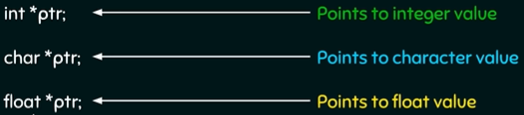
\includegraphics[width=180 pt]{Pointer which is points to.png}
\end{center}
We can assign values to the pointer by \textcolor{red}{address\_of} operator. Which is \textcolor{red}{Ampersand}.
\begin{center}
	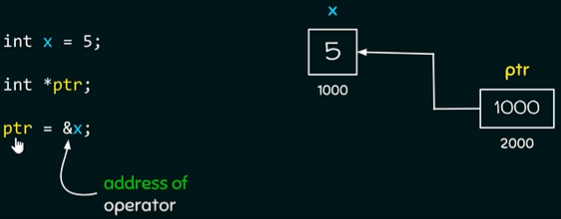
\includegraphics[width=180 pt]{Assigning address to the pointer.png}
\end{center}
We know that, pointer is also a variable so that it also takes place in memory and then store address of another variable in it.

\subsection{Dynamic Memory Allocation}
Dynamic memory allocation in C/C++ refers to performing allocate memory manually by the programmer. Dynamically allocated memories allocated on \textbf{HEAP}.\\
\begin{tcolorbox}
	Dynamic memory allocation is the process of assigning memory cell during execution time of the program.
		\begin{tcolorbox}[width=6.5cm, colframe=red!90]
			Run-Time memory allocation.
		\end{tcolorbox}
\end{tcolorbox}

\subsubsection{New and Delete operations}
Where C uses \textcolor{red}{malloc(}) function for dynamically allocate memory and free() for remove this. \textcolor{red}{malloc()} is a system function which allocates memory on the heap and returns a pointer to the new block. C++ standard supports these functions but also have two extra operator namely new and delete for performing same task in a better and easier way.\\
\textbf{New} is an operator which denotes a request to memory for allocate space on Heap. \textbf{New} operators initializes the memory and returns address of the newly allocated and initialized memory to the pointer variable.

\section{Illustration of C++ code}
 If there some problem with the STL of C++, then made own build in functions.
 Text before \dots
 \LaTeX
 \begin{lstlisting}
 for(int i=0; i<iterations; i++)
 {
  do something;
 }
 \end{lstlisting}
 Text after it \dots
 \subsection{Finding maximum element from an array of size n}

\begin{lstlisting}[frame=shadowbox, rulesepcolor=\color{blue!80}]
int MaxEle(int arr[], int n)
{
    int i, a=0;
    for(i=0; i<n; i++)
    {
        a = max(a, arr[i]);
    }
    return a;
} 
\end{lstlisting}

\subsection{Counting selected element from an array}
 
\begin{lstlisting}[frame=shadowbox, rulesepcolor=\color{green!80}]
int Count(int arr[], int n, int value)
{
    int c=0, i;
    for(i=0; i<n; i++)
    {
        if(arr[i]==value)
        {
            c++;
        }
    }
    return c;
}
 \end{lstlisting}
 
\subsection{Divide function by string}

\begin{tcolorbox}
\begin{lstlisting}
#include <bits/stdc++.h>
using namespace std;

string divide(string &ns, int &dividor, int &rem)
{
    int i;
    string result;
    rem = ns[0] - '0';
    for (i = 1; i < ns.size(); i++)
    {
        if (rem < dividor)
        {
            rem = rem * 10 + (ns[i] - '0');
            i++;
        }
        result.push_back(rem / dividor + '0');
        rem %= dividor;
    }
    return result;
}

int main()
{
    string ns;
    int dividor, rem;
    rem = 0;
    cin >> ns >> dividor;
    cout << ns << "/" << dividor << " = "
         << divide(ns, dividor, rem) << endl;
    cout << "Reminder: " << rem << endl;
}
\end{lstlisting}
\end{tcolorbox}

\subsection{BitWise Operator}
Works at bit-level.
Do we know that? Every odd number in binary representation hold true bit in first and last bit.
\begin{table}
\caption{Odd numbers in binary}
 \begin{center}
  \begin{tabular}{c c}
  ODD Decimal & in Binary\\
  1 & 1\\
  3 & 11\\
  5 & 101\\
  7 & 111\\
  9 & 1001 
  \end{tabular}
 \end{center}
\end{table}
Is it clear? OK. As reverse way, all even number in binary representation hold first true bit and false in last. For the sake of illustration:-
\begin{table}
\caption{Even numbers in binary}
 \begin{center}
  \begin{tabular}{c c}
  EVEN Decimal & in Binary\\
  2 & 10\\
  4 & 100\\
  6 & 110\\
  8 & 1000\\
  10 & 1010 
  \end{tabular}
 \end{center}
\end{table}

Bitwise operators works on binary bits of given number.
\subsubsection{Some Interesting things about bitwise operator}
\begin{enumerate}
 \item 'N' is a given number, N will be odd if bitwise operation between N and 1 is 1. Means: (N\&1)=1, if N if odd. Else 0 if N is even.
 \item The left shift and right shift operators should not be used for negative numbers.
 \item We can find odd occurring number in an array by XOR.\\
 \begin{lstlisting}
 s;kldf
 \end{lstlisting}
\end{enumerate}

\subsection{Structure}
\begin{lstlisting}[basicstyle=\footnotesize, frame=single, frameround=tftf, numbers=left, stepnumber=2, numberfirstline=false, caption=Structure in C/C++]
#include<bits/stdc++.h>
using namespace std;

///Now we gonna learning structure in C++.
/*
    Sometimes we need a group of different types
    data in one specific class collection. For get
    released from this problem, C and C++ provides
    a new user-defined data-type.
    To define a structure, use the keyword "struct".
*/
struct student
{
    /*
        All members of struct is generally public.
    */
    int ID;
    string sex;
};

int main()
{
    /*
        Let's declare a student struct of class 6 that
        has 3 students.
        First student(class6[0]) has 33 as roll.
    */
    student class6[3];
    class6[0].ID=33;
    class6[1].ID=34;
    cout << class6[0].ID << endl;
    cout << class6[1].ID << endl;
    student kiron;
    cin >> kiron.ID;
    cout << "Kirons id " << kiron.ID << endl;
    cin >> kiron.sex;
    cout << "Kirons sex " << kiron.sex << endl;

    /*
        Let's declare a pointer of type student.
        That can store address of student type variables.
    */
    student *ptr;
    /*
        Now This pointer will store address of kiron's all
        member function.
    */
    ptr = &kiron;
    /*
        Now ptr points to all member variable of
        struct variable kiron.
    */

    kiron.ID=65;
    ptr->sex="Male";
    cout << ptr->ID << endl;
    cout << kiron.sex << endl;
    /*
    	Arrow operator is used for access by pointer.
    */
}
\end{lstlisting}

\subsection{How to check efficiently that a number is palindrome or not}
\href{https://leetcode.com/articles/palindrome-number/}{Link}\\
\begin{flushleft}
\textbf{Intuition}
The first idea that comes to mind is to convert the number into string, and check if the string is a palindrome, but this would require extra non-constant space for creating the string which is not allowed by the problem description.\linebreak
\linebreak
Second idea would be reverting the number itself, and then compare the number with original number, if they are the same, then the number is a palindrome. However, if the reversed number is larger than \textbf{int.MAX}, we will hit integer overflow problem.
\linebreak
\linebreak
Following the thoughts based on the second idea, to avoid the overflow issue of the reverted number, what if we only revert half of the \textbf{int} number? After all, the reverse of the last half of the palindrome should be the same as the first half of the number, if the number is a palindrome.
\linebreak
\linebreak
For example, if the input is 1221, if we can revert the last part of the number "1221" from "21" to "12", and compare it with the first half of the number "12", since 12 is the same as 12, we know that the number is a palindrome.
\end{flushleft}
\textbf{Algorithm}\\
First of all we should take care of some edge cases. All negative numbers are not palindrome, for example: -123 is not a palindrome since the '-' does not equal to '3'. So we can return false for all negative numbers.
\linebreak
\linebreak
Now let's think about how to revert the last half of the number. For number 1221, if we do 1221 \% 10, we get the last digit 1, to get the second to the last digit, we need to remove the last digit from 1221, we could do so by dividing it by 10, 1221 / 10 = 122. Then we can get the last digit again by doing a modulus by 10, 122 \% 10 = 2, and if we multiply the last digit by 10 and add the second last digit, 1 * 10 + 2 = 12, it gives us the reverted number we want. Continuing this process would give us the reverted number with more digits.
\linebreak
\linebreak
Now the question is, \textit{how do we know that we've reached the half of the number?}
\linebreak
\linebreak
Since we divided the number by 10, and multiplied the reversed number by 10, when the original number is less than the reversed number, it means we've processed half of the number digits.

 \section{STL Map}
 Map is a associated container of C++ STL(Standard Template Library). A map variable has two part,
 
 \begin{enumerate}
  \item Key
  \item Value
 \end{enumerate}
 
 \href{https://www.geeksforgeeks.org/map-associative-containers-the-c-standard-template-library-stl/}{\textcolor{blue}{Geeks for Geeks}}: Maps are associative container that stores data in a mapped fashion. No two map values can have same key values.\\
 
 \begin{lstlisting}
  #include<map>
  // Declaring Map
  map<int, int> mp; // mp: map name.
  // First one is keyvalue, second one is mapvalue.
  
  // Insert elements in random order.
  mp.insert(pair<int, int>(1, 40));
  
  //Creating map iterator:
  map<int, int> :: iterator it;
  
  //Accessing the map data:
  it -> first; // Refer keyvalue.
  it -> second; // Refer mapvalue.
 \end{lstlisting}
 
  \subsection{Map member function}
   1. insert() :- The key must be unique.
   
   \begin{lstlisting}
   //Syntax:
    map_name.insert({key, value});
    
    //e.g.
    map<int, int> mp;
    mp.insert({1, 40});
   \end{lstlisting}
   
   2. count() :-
      
   \section{STL pair}
   
   \begin{lstlisting}
#include<iostream>

/*For pair access, include this header file.
utility is a STL.*/
#include<utility>
using namespace std;

int main()
{
    pair<int, int>p1;
    p1.first = 1;
    p1.second = 2;
    cout << p1.first << " " << p1.second << endl;

    ///Declaring pair array with the size 4.
    pair<int, int>p[4];
    //All pair value assigned to 0 automatically.

    p[0].first=1;
    p[0].second=2;
    cout << p[0].first << " " << p[0].second << endl;

    /*Here we not assigned any value to the pair p[1] and p[2].
    So there will print 0*/
    cout << p[1].first << " " << p[1].second << endl;
    cout << p[2].first << " " << p[2].second << endl;

    /*
     Member function: make_pair().
     This member function assign values to pair directly.
     Thats mean, this is more sexy.
     Syntax: pair_name = make_pair(value1, value2);
    */
    pair<string, double> ps;
    ps = make_pair("My S.S.C result: ", 4.56);
    cout << ps.first << ps.second << endl;

    /*
     Operating pairs.
     1. (==) comparison.
        It will return 1 is those pairs both values are equal otherwise 0.
        As same for all other comparisons like >=, <=, != etc.
    */
    pair<int, int> pair1, pair2, pair3;
    pair1 = make_pair(1, 4);
    pair2 = make_pair(1, 4);
    pair3 = make_pair(2, 4.1);
    /*No matter what type value we assigned,
    It will type casted automatically by the data type as we declared.
    So it will be same as (2, 4).
    */

    if(pair1==pair2)
    {
        cout << "Pairs are same" << endl;
    }
    cout << (pair1==pair2) << endl;
    if(pair1!=pair3)
    {
        cout << "pair1 and pair3 are not same" << endl;
    }
    else
    {
        cout << "pair1 and pair3 are same" << endl;
    }

    /*
     swap()
     Syntax: pair1.swap(pair2);
     It will swap values of both pair.
     swap pair1.first with pair2.first then
     swap pair1.second with pair2.second
    */
    pair1.swap(pair3);
    cout << pair1.first << " " << pair1.second << endl;
    
    /*
     swap() isn't working in code::blocks but in other
     online compiler, it works perfectly.
     */
}


   \end{lstlisting}
   
\section{STL List}
Lists are sequence of elements stored in a linked list. Compared to vectors, they allow fast insertions and deletions, but slower random access.\\
\subsection{Member Functions of List}
\begin{tabular}{|c c|}
\hline
Function & Task\\
\hline
assign & assign elements to list\\
\hline
begin & returns an iterator to the beginning of the list\\
\hline
back & returns a reference to last element of list\\
\hline
clear & removes all elements from the list(Clears the list)\\
\hline
empty & returns true if list is empty\\
\hline
end & returns an iterator just past the last element of a list\\
\hline
erase & remove specific element from list\\
\hline
front & returns a reference to the first element of a list\\
\hline
insert & insert elements into the list\\
\hline
max\_size & returns the maximum number of elements that the list can hold\\
\hline
merge & merge two lists\\
\hline
push\_back & add an element at end of the list\\
\hline
push\_front & add an element at beginning of the list\\
\hline
pop\_back & removes the last element of the list\\
\hline
pop\_front & remove first element of the list\\
\hline
rbegin & return reverse begin iterator\\
\hline
rend & return reverse end iterator\\
\hline
remove & remove elements from list\\
\hline
remove\_if & remove element conditionally\\
\hline
resize & change size of the list\\
\hline
reverse & reverse the list\\
\hline
size & returns the numbers of elements present in the list\\
\hline
sort & sorts the list in ascending order\\
\hline
splice & merge the lists in constant time\\
\hline
swap & swap two list with each other with all elements\\
\hline
\textcolor{red}{unique} & removes duplicate element\\
\hline
\end{tabular}
\subsection{Discuss}
\begin{lstlisting}
vector<int> v(5, 42);
\end{lstlisting}
It will produce a vector named v with five times 42.\\
\begin{lstlisting}[frame=shadowbox, rulesepcolor=\color{green!60}]
#include<bits/stdc++.h>
using namespace std;

int main()
{
    vector<int> v(5, 42);
    for(int i=0; i<v.size(); i++)
    {
        cout << v[i] << " ";
    }
    cout << endl;
}
\end{lstlisting}
\begin{tcolorbox}[colback=black!3]{Output:}
42 42 42 42 42
\end{tcolorbox}
\subsection{assign}
assign member function is used assign values from one to another.\\
\begin{lstlisting}[frame=shadowbox, rulesepcolor=\color{green!60}]
#include<bits/stdc++.h>
using namespace std;

int main()
{
    vector<int> v1;
    for(int i=0; i<10; i++)
    {
        v1.push_back(i);
    }
    vector<int> v2;
    v2.assign(v1.begin(), v1.end());
    for(int i=0; i<v2.size(); i++)
    {
        cout << v2[i] << " ";
    }
    cout << endl;
}
\end{lstlisting}

\section{STL Stack}
\begin{lstlisting}[caption=Stack, frame=shadowbox, rulesepcolor=\color{green!70}]
#include<iostream>
#include<stack>
using namespace std;

/*
 Stacks are a type of container adaptors with LIFO(Last IN First Out).
 So we can say, stack is Stup.
*/

int main()
{
    /*Let's create a stack of int type.*/
    stack<int> s;

    /*Member function push() will add the new element at the top
    of the stack.
    Time complexity O(1)*/
    s.push(10);
    s.push(9); /*9 stored above of 10*/
    s.push(8);
    s.push(1); /*Now 1 is the top most element.*/

    /*Algorithmic function size() returns current size of
    this stack.*/
    cout << s.size() << endl;

    /*Member function top() will return topper element or that element
    we entered last.
    For this example, it is 1*/
    cout << s.top() << endl;

    /*Member function pop() will delete the topmost element.*/
    s.pop();
    
    /*After removing topmost element,
    present topmost element is 8*/
    cout << s.top() << endl;
    
    /*After removing one element,
    current size of stack is 3*/
    cout << s.size() << endl;

    /*Algorithmic function empty() will return true if there is
    no element at the stack.*/
    if(!s.empty())
    {
        cout << "Stack is not empty" << endl;
    }

    return 0;
}
\end{lstlisting}
\begin{center}
\begin{tcolorbox}[enhanced, title=Output,
attach boxed title to bottom center, width=3.9 cm]
4\\1\\8\\3\\Stack is not empty
\end{tcolorbox}
\end{center}
   
\section{Power of 2}
\subsection{Binary Transform of \textbf{$2^n$}}
Look at the table:-\\(\LaTeX  provides a large set of tool for formatting tables)\\

\begin{center}
\begin{tabular}{||c | c | c | c||}
\hline
$2^n$ & Decimal & Binary & Seems like\\
\hline\hline
$2^0$ & 1 & 1 & $10^0$\\
\hline
$2^1$ & 2 & 10 & $10^1$\\
\hline
$2^2$ & 4 & 100 & $10^2$\\
\hline
$2^3$ & 8 & 1000 & $10^3$\\
\hline
$2^4$ & 16 & 10000 & $10^4$\\
\hline
$2^5$ & 32 & 100000 & $10^5$\\
\hline
\end{tabular}
\end{center}

It's clear that power of 2 in binary holds just one and only one true bit. So, we can simply say that, a number will be power of 2 if its binary holds just one true bit at first.

\subsection{Algorithm}
\begin{tcolorbox}
\begin{enumerate}
\item Take a decimal number string "ds".
\item Convert the number into binary string by a function.
 \begin{enumerate}
 \item Return binary string name such as "bs".
 \end{enumerate}
\item Start checking from the index 1.
\item If find out a true bit
 \begin{tcolorbox}
 return false;
 \end{tcolorbox}
 That mean, this is not power of 2.
\item Else: Till to end, there is no true bit.
 \begin{tcolorbox}
 return true;
 \end{tcolorbox}
 That mean, this is power of 2.
\end{enumerate}
\end{tcolorbox}

\section{Linked Lists}
Reference: \href{https://www.youtube.com/watch?v=njTh_OwMljA}{\textcolor{red}{Hacker Rank}}\\
Today we are going talk about linked lists. It's essentially just a sequence of the element, where each element links to the next elements which next element links to the next elements. A linked list can contain pretty much any kind of data - string, char, int. The elements can be sorted or unsorted, duplicates or unique. If we want to access element from linked list, we need linear time where array give us constant time, because for access array element, just boom, instantly do that. There are two type of linked list. Singly linked list and doubly linked list. Doubly linked list is a alternate version of singly linked list and access of elements from doubly link list is pretty much easy. One doubly linked list element has two part. One is previous node a second is next element. That mean, each elements having a link to the next element, each elements also linked to the previous element. So, for certain operations, this can be quite handy.\\
\href{https://www.geeksforgeeks.org/linked-list-set-1-introduction/}{\textcolor{red}{Geeks for Geeks}}\\
Advantages over arrays:-
\begin{itemize}
	\item Dynamic size
	\item Ease of insertion and deletion
\end{itemize}
Drawbacks:-
\begin{enumerate}
	\item Random access not allowed. We have to access elements sequentially from the first node called HEAD. So we can't do binary search with linked lists efficiently with its default implementation.
	\item Extra memory allocation required for a pointer with each elements of the list.
	\item As array, elements are not stored in contiguous location.
\end{enumerate}
Representation:-\\
A linked list is represented by a pointer to the first node of the linked list. If the linked list is empty, then the value of the HEAD is NULL. A node consist with two parts:-
\begin{itemize}
	\item Data
	\item Reference to the next node, i.e. pointer*.\footnote{\texttt{\hspace{0.4 cm}*A pointer is a special type of variable that stores memory address of another variable. Pointer is declared by asterisk sign before which variable we want to declare that it is a pointer. We can access address of a variable by using ampersand sign before it.}}
\end{itemize}

Let's create a user-defined data-type for build a node. A node has two part, one data and another pointer that points to the next node(That also has two part). So, the pointer must be such type that holds the next node(with two part). Means the pointer must be a node object.
IN C, node represented by struct. IN object-oriented language, it does with Class. Here the implementation in C++.
\begin{lstlisting}[caption=Node Class]
	class Node
	{
	 public:
	 	int data;
	 	Node *next;
	};
\end{lstlisting}
Block illustration of this code:-\\
\tikz
{
	\draw (0, 0)--(1, 0)--(1, -0.5)--(0, -0.5)--(0, 0);
	\draw (0.5, 0)--(0.5, -0.5);
	\draw[->] (1, -0.25)--(1.5, -0.25);
	\draw (1.5, 0)--(2.5, 0)--(2.5, -0.5)--(1.5, -0.5)--(1.5, 0);
	\draw (2, 0)--(2, -0.5);
	\draw[->] (2.5, -0.25)--(3, -0.25);
	\draw (3, 0)--(4, 0)--(4, -0.5)--(3, -0.5)--(3, 0);
	\draw (3.5, 0)--(3.5, -0.5);
}

 \section{Fortran}
 \textbf{Fortran} means Formula Translation. This is a general-purpose, compiled imperative programming language that's are specially suited to numeric computation and scientific computing, originally developed by IBM.\\
 (\textbf{IBM} - \textit{International Business Machines Corporation.})

\section{Python}
 In Linux and Mac operating systems, python are already installed. For install in windows, first we need to go \href{https://www.python.org/}{\textcolor{blue}{Pythons Official Website}}. Then download python and install.\\
\subsection{Why we use Python}
 Easy to learn, easy to use
 Popular in web development
 Can create a full web application
 
\chapter{Java}
Java is an open source high-level, general-purpose(hard \& used to develop any kind of programs), object oriented language. If you wanna be a software developer than you must learn that 4 languages:-
\begin{enumerate}
	\item Python
	\item Java
	\item JavaScript
	\item C / C++
\end{enumerate}
In those, Java is second dominant (and popular also) language that you must learn if you wanna be a platform-independent developer. Also:-
\begin{itemize}
	\item[$\rightarrow$] Java has huge online community for getting help.
	\item[$\rightarrow$] Can be used in android development that is most preferable thing today.
\end{itemize}

\paragraph{Gosling explains his motivation for creating \textbf{JAVA}:}
James Gosling, father of \textbf{JAVA}. It is one of the world's most widely used programming language. It used over ten billion of devices and become central to the development of Android at Google. According to \textbf{Oracle}, there are $51$ billion active Java Virtual Machines deployed globally.

Java has two types of error. Syntax error and Semantic error. Syntax error is grammatical error and semantic error is that the line has no meaning.
\begin{itemize}
	\item[$\rightarrow$] "I are playing" - that's the syntax error.
	\item[$\rightarrow$] "He is hello" - this line has no meaning, semantic error.
\end{itemize}
\begin{center}
	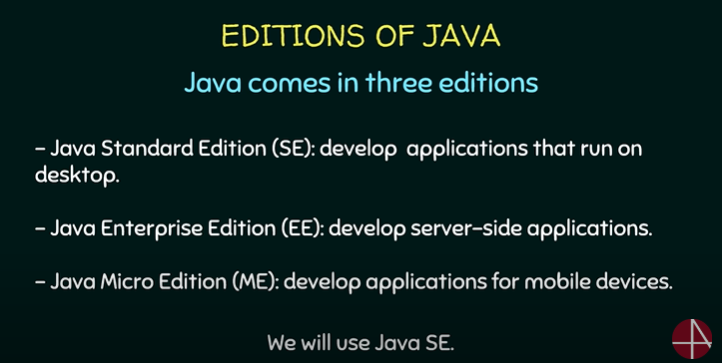
\includegraphics[width=200pt]{Editions of Java.png}
\end{center}

\section{IntelliJ IDEA: The IDE} % All OK.
\begin{wrapfigure}{r}{0.25\textwidth}
	
\includegraphics[width = 0.9\linewidth]{IntelliJ IDEA user interface.png}
\end{wrapfigure}

\textbf{IntelliJ IDEA} is the greatest \textbf{IDE} for writing and compiling Java source codes. Here in table \ref{IntelliJ IDEA:1} has some command and shortcuts of \textbf{IntelliJ IDEA} that are applicable to windows operating system.

\begin{center}
\rowcolors{3}{green!35}{green!70}
\arrayrulecolor{white}
	\begin{longtable}{|| m{1 em} || m{15 em} m{17 em} ||}
	\label{IntelliJ IDEA:1}\\
		\hline\hline
		\rowcolor{teal!20}
		\multicolumn{3}{c}{\textbf{\textsf{\textcolor{black}{IntelliJ IDEA Commands and Shortcuts}}}}\\
		\hline\hline
		1 & Debug Program & shift + f9\\
		\hline
		2 & Run Program & shift + f10\\
		\hline
		3 & Format Codes & ctrl + alt + L\\
		\hline
		4 & public static void main() & main / psvm\\
		\hline
		5 & System.out.println() & sout\\
		\hline
		6 & To warp a code block in a construct & ctrl + alt + T\\
		\hline
		7 & Search anything in project & double click shift (For a technical reason, I turned off the system)\\
		\hline
		8 & Invoke commit changes dialog & ctrl + K\\
		\hline
		9 & Select several words and edit together & press and hold shift + alt and double click on the word.\\
		\hline
		10 & Fill the code construct & start typing method declaration and press ctrl + shift + enter\\
		\hline
		11 & Join two statement in one line and remove unnecessary spaces & ctrl + shift + J\\
		\hline
		12 & Jump highlighted syntax error & f2 / shift + f2\\
		\hline
		13 & ctrl + shift + E & recently viewed or changed code fragment\\
		\hline
		14 & Change name of the function from main method & highlight method name then press shift + f6 and re-write\\
		\hline
		\rowcolor{red}
		15 & Quick scheme & view | Quick Switch Scheme or ctrl +  \\
		\hline
		16 & To evaluate any expression while debugging program & select the expression in the editor and press Alt + F8\\
		\hline
		17 & Create a new class & alt + ins (Now, not working perfectly)\\
		\hline
		18 & To see all the live template that are valid for this current method or context & ctrl + J (Close this by pressing "esc")\\
		\hline
		19 & Complete syntax with dot from code completion helper(highlighted) & ctrl + dot\\
		\hline
		20 & To close all editor tabs except current one & keep alt pressed and click cross button of current tab\\
		\hline
		21 & To see how to call an action & ctrl + shift + A\\
		\hline
		22 & To select multiple fragment in column mode & press alt + shift + insert and then hold ctrl + shift + alt and drag the mouse\\
		\hline
		23 & Rename an identifier and change all uses of it & Look at the leftmost side(gutter), here is a pencil marker. Click on this and click again Rename.\\
		\hline
		24 & To select a block of code & Double click of its opening brace.\\
		\hline
		25 & Invoke rename action box & mark down the field and press shift + f6\\
		\hline
		26 & Move statement up/down in current block only & put cursor at the end of the statement and hold shift + ctrl then press uparrow/downarrow\\
		\hline
		27 & Move line up/down at any place & shift + alt + up/down\\
		\hline
		28 & To scroll a file horizontally & Turn the mouse wheel while keeping Shift pressed\\
		\hline
		29 & Compare to different directories & select the file on form project (Press and hold shift and then one click on the directory) and press ctrl + D\\
		\hline
		30 & To delete the whole line at the caret & ctrl + Y\\
		\hline\hline
	\caption{Commands and Shortcuts: Intellij IDEA}
	\end{longtable}
	
\end{center}

\section{Syntax Difference between \textcolor{blue!90}{C++} and \textcolor{blue!90}{Java}}
\begin{table}[h!] % h! : In-place command.
	\arrayrulecolor{black}
	\centering
	\begin{tabular}{|| c | c ||}
		\hline
		\textbf{\textcolor{blue}{C++}} & \textbf{\textcolor{blue}{Java}}\\
		\hline\hline
		string & String\\
		\hline
		int main() & public static void main()\\
		\hline
		empty() & isEmpty()\\
		\hline
		vector & ArrayList()\\
		\hline
	\end{tabular}
	\caption{Syntax Difference between \textcolor{blue!90}{\huge C++} and \textcolor{blue!90}{\huge Java}}
\end{table}

\section{Object Oriented Programming (OOP) with \textbf{JAVA}}
As I mentioned, Java is full object oriented language and do not provide low level programming features like pointer, operator overloading etc. as C / C++ does. Every byte of code of Java are written in a class with same name of that file. Now, what is object? An object is a collection of data (of primitive type) belongs to a class and that class provides methods for manipulate this object. So, Java is "object-oriented" means it uses object to represent data and provide methods related to them. To create a new object in Java, must use \textcolor{blue}{new} keyword. Java has a huge amount of built-in classes, \textbf{Point} and \textbf{Rectangle} are two of them. You can see details of that two classes from oracles Java documentation. As we know from previous section, some of same type classes are wrapped in a package. Point class is belongs to \textbf{awt} package of Java source code library. Variables that belong to an object are usually called \textbf{attribute}, but you might also see them called \textbf{fields}. Both are correct. To access an attribute of an object, Java uses \textbf{dot notation}. Syntax:-\hfill
\begin{lstlisting}[language = java]
	dataType variable = objectName.attribute;
\end{lstlisting}
Objects are pass by reference to the method. In Java, keyword \textcolor{blue}{null} means "No Objects". When you try to use a null value, \textbf{NullPointerException} will be thrown. But you can return or send a null value to a method.

\section{Arrays Class}
Arrays class are used to manipulate arrays. Arrays class is a member of the java Collections Framework. We can initialize Array like this, \texttt{int anArray[];} which is not conventional way.\\
Iterate over array by a stream:\\
\texttt{\footnotesize Arrays.stream(new int[] {1, 2, 3}).forEach(n -> System.out.print(n + " "));}
\subsection{parallelSort() Method}
Java 8 introduced a new method called \textbf{parallelSort()} in java.util.Arrays class. If uses parallel sort algorithm. This method uses "MultiThreading" which makes the sorting faster as compared to normal sorting method. This is a void method. Time complexity $O(n\log(n))$
\paragraph{Algorithm for parallelSort():}
	\begin{enumerate}
		\item The array is divided into sub-arrays and that sub-array is again divided into their sub-arrays. Until the minimum level of detail in a set of array.
		\item Arrays are sorted individually my multiple thread.
		\item This algorithm uses Frok / Join concept for sorting.
		\item Sorted sub-arrays are then merged.
	\end{enumerate}

\section{Matcher Class}
Reference: \href{https://docs.oracle.com/javase/7/docs/api/java/util/regex/Matcher.html}{Oracle Help Center}\linebreak
I have written some descriptions for this class in my Java notebook.

\paragraph{Package}
java.util.regex
\paragraph{Properties}
An engine that perform match operations on a character sequence by interpreting patter(Such a regular expression or regex.)

\section{Interface}
Interface is a feature that implements most futuristic class. In java programming language, an interface is a reference type, similar to a class, that can contain only constants, method signatures, default methods, interfaces cannot be instantiated - they can only be implemented by classes or extended by other interfaces. Extension is discussed later in this lesson. All method had just signature but not method body. Methods signature are terminated with a semicolon.

\section{Anonymous Class}
Anonymous class enables you to make your code more concise. They enable you to declare and instantiate a class at the same time. They are look like local classes except that they don't have a name.\hfill
Use them if you need to use a local class only once.

\section{Lambda Expression}
Lambda Expression enables you to pass functionality as an argument to another method. Such as, what action should be taken when someone clicks a button.
\paragraph{Note of Collection:}A \textcolor{blue}{Collection} is an object that groups multiple elements into a single unit by a wrapper class for primitives and instant class for local class objects. Collections are used to store, retrieve, manipulate and communicate aggregate data. As, a \textcolor{blue}{List} is an \textcolor{blue}{Collection} of ordered type.

\section{Object Ordering}
\begin{framed}
	\begin{lstlisting}[language = java]
		Collections.sort(list)
	\end{lstlisting}
\end{framed}
\paragraph{Starting:}
\begin{multicols}{2}
There is an interface named \textit{\textcolor{blue}{Comparable}} and has a \textit{\textcolor{blue}{compare}} method at this. we can use(override) this method for our own manipulation of sorting / ordering. \textsf{Comparable} implementations provide a \textit{natural ordering} for a class, which allows objects of that class to be sorted automatically.\linebreak
If you try to sort a list, which don not implement Comparable, will throw a \textbf{\textcolor{blue}{ClassCastException}}. Similarly, \textit{Collections.sort(list)} will throw the same exception if we try to sort that list whose elements cannot be compared to one another.
\end{multicols}
\begin{quotation}
	Elements that can be compared to one another are called \textit{mutually comparable}.
	\begin{flushright}
		- Oracle
	\end{flushright}
\end{quotation}

\subsection{Implement own comparable type}
The comparable interface consist of the following methods:
\begin{lstlisting}
	public interface Comparable<T>
	{
		public int compareTo(T o);
	}
\end{lstlisting}

This method compares the receiving object with the specified object and returns negative, zero or positive value depending on whether the receiving object is less than, equal or greater than the specified object.
\begin{lstlisting}[language = java, backgroundcolor = \color{white}]
public class Name implements Comparable<Name>
{
    private final String firstName, lastName;

    public Name(String firstName, String lastName)
    {
        if (firstName == null || lastName == null)
            throw new NullPointerException();

        this.firstName = firstName;
        this.lastName = lastName;
    }

    public String firstName() {return firstName;}
    public String lastName() {return lastName;}

    public boolean equals(Object o)
    {
        if (!(o instanceof Name))
            return false;

        Name n = (Name) o;
        return n.firstName.equals(firstName) && n.lastName.equals(lastName);
    }

    public int hashCode()
    {
    	return 31 * firstName.hashCode() + lastName.hashCode();
    }
    public String toString() {return firstName + " " + lastName;}

    public int compareTo(Name n)
    {
        int lastCmp = lastName.compareTo(n.lastName);
        return (lastCmp != 0 ? lastCmp : firstName.compareTo(n.firstName));
    }
}
\end{lstlisting}

\subsection{Comparators}
What if you want to sort some objects in an order other than their natural ordering? Or what if you want to sort some objects that don't implement Comparable? To do either of these things, you'll need to provide a Comparator - an object that encapsulates an ordering. The Comparator interface consists of a single method:
	\begin{lstlisting}
		public interface Comparator<T>
		{
			int compare(T o1, T o2);
		}
	\end{lstlisting}

The \textit{compare} method returns less than zero, zero or greater than zero depending on whether the first argument is less than, equal or greater than the second.
\paragraph{By GeeksforGeeks:}
A \textit{comparator} is an interface\footnote{That just had a face, no body.} that used to order the objects of user-	defined classes. A \textit{comparator} object is capable of comparing two objects of two different classes. Suppose we have an "ArrayList" of objects containing fields like \textsc{Name, Roll, Section} and we need to sort the "ArrayList" based on \textsc{Roll}. We can do this by:
	\begin{enumerate}
		\item[Method 1:] One obvious approach is to write our own "sort()" function using one of the standard algorithm. This approach require rewrite the entire function.
		\item[Method 2:] Using \textit{comparator} interface\footnote{Present in java.util package.}. It contains two method signature:-
		\begin{enumerate}
			\item compare(Object o1, Object o2);
			\item equals(Object element);
		\end{enumerate}
	\end{enumerate}
	
\subparagraph{How does "Collections.sort()" work?}
Internally the "sort()" method calls Compare method of that class and asks for "which is grater?". Then compare method returns $-1, 0$ or $1$ based on compared object. It uses this result to then determine if they should be swapped for its sort.
\subparagraph{A working program:}
A working program from geeksforgeeks
\begin{lstlisting}[language = java, caption = Comparator for sorting Student class, backgroundcolor = \color{white}]
class Student
{
    String name, address;
    int roll;

    public Student(String name, int roll, String address)
    {
        this.name = name;
        this.roll = roll;
        this.address = address;
    }

    public String toString()
    {
        return this.name + " " + this.roll + " " + this.address;
    }
}

class SortByName implements Comparator<Student>
{
    public int compare(Student s1, Student s2)
    {
        return s1.name.compareTo(s2.name);
    }
}

class SortByAddress implements Comparator<Student>
{
    public int compare(Student s1, Student s2)
    {
        return s1.address.compareTo(s2.address);
    }
}

class Main
{
    public static void main(String[] args)
    {
        ArrayList<Student> list = new ArrayList<>();
        list.add(new Student("Kiron", 65, "Madaripur"));
        list.add(new Student("Miron", 73, "Faridpur"));
        list.add(new Student("Chiron", 11, "Dhaka"));

        Collections.sort(list, new SortByName());
        for (int i = 0; i < list.size(); i++)
            System.out.println(list.get(i));

        System.out.println();
        Collections.sort(list, new SortByAddress());
        for (int i = 0; i < list.size(); i++)
            System.out.println(list.get(i));
    }
}
\end{lstlisting}

\begin{tcolorbox}[enhanced, title = Output, attach boxed title to top left, width = 5 cm]
	Chiron 11 Dhaka\\
	Kiron 65 Madaripur\\
	Miron 73 Foridpur\\
\vspace{2.5 mm}
	Chiron 11 Dhaka\\
	Miron 73 Foridpur\\
	Kiron 65 Madaripur\\
\end{tcolorbox}

Just change the return value inside compare method, that will allow us to sort objects in required manner. e.g. for descending order, swap the position of objects.

\paragraph{Again Oracle:}
\section{Math Class}
\subsection{Beyond Math Class}
The "Math" class in \textit{java.lang} package provides methods and constants for doing more advance mathematical computation. All the methods in "Math" class are "static", so they can be called directly. Using the \textbf{\textcolor{blue}{static import}} language feature, you don't have to write Math in front of every math function.
\begin{lstlisting} [language = java]
	import static java.lang.Math.*;
\end{lstlisting}

* will import all the methods from the "Math" class.\\
Now we can write code like this:
\subsection{Constants and Basic Methods}
The class contains two constants:
	\begin{enumerate}
		\item[Math.E] Base of natural logarithms.
		\item[Math.PI] Ratio of the circumference of a circle to its diameter.
	\end{enumerate}
	
This class also includes more than 40 static methods.
	\begin{enumerate}
	
\subsection{Random Numbers}
The random() method returns a pseudo-randomly selected number between 0.0 and 1.0
	\begin{lstlisting} [language = java]
		
	\end{lstlisting}
		\item[primitive abs(primitive arg)] Returns the absolute value of "arg".
		\item[ceil()]
		\item[floor()]
		\item[double rint(double d)] Returns the integer that is closest in value to the argument as double.
		\item min(a, b);
		\item max(a, b);
		\item double exp(double d);
		\item double log(double d);
		\item pow(base, exponent);
		\item sqrt(double d);
		\item All trigonometric methods.
		\item [double atan2(double y, double x)] Converts rectangular coordinates (x, y) to polar coordinate (r, $\theta$) and returns $\theta$.
		\item double toDegrees(double d);
		\item double toRadians(double d);
	\end{enumerate}
	con(angle);
\end{lstlisting}

\section{Graph}

\subsection{Representation}

\paragraph{What is graph:}
Graph is a collection of nodes / vertices(\textbf{V}) and edges(\textbf{E}) placed between them. Represented as: $$G = (V, E)$$ We can traverse vertices through edges. These edges might be weighted or non-weighted.

\subparagraph{There are two kinds of graphs:}
	\begin{itemize}
		\item[Un-directed:] Not direction specified. We can traverse either direction between two vertices.
\tikzset
{
	VertexForGraph/.style = {draw, circle, very thick, black, fill = teal!30}
}
\begin{center}
	\tikz
	{
		\node(0) at (-1, 2) [VertexForGraph] {A};
		\node(1) at (2 ,2) [VertexForGraph] {B};
		\node(2) at (4.5, 0.5) [VertexForGraph] {C};
		\node(3) at (2, -1) [VertexForGraph] {D};
		\node(4) at (-1, -1) [VertexForGraph] {E};
	
		\draw (0) -- (1);
		\draw (1) -- (2);
		\draw (1) -- (3);
		\draw (1) -- (4);
		\draw (2) -- (3);
		\draw (3) -- (4);
		\draw (4) -- (0);
	}
\end{center}
		\item[Directed:] Can traverse only in the specified direction between that two vertices.
	\end{itemize}
	
\subparagraph{Two common ways to represent a graph:}
	\begin{itemize}
		\item Adjacency Matrix
		\item Adjacency List
	\end{itemize}

\paragraph{Adjacency Matrix:}
Adjacency matrix is a 2D array which had the size of\\$(V$ $*$ $V)$, where $V$ are the number of vertices in the graph. Adjacency matrix is symmetric if the graph is un-directed. Here is the adjacency matrix for above graph:
	\begin{table}[h!]
		\centering
		\begin{tabular}{c c c c c c}
			  & A & B & C & D & E\\
			A & 0 & 1 & 0 & 0 & 1\\
			B & 1 & 0 & 1 & 1 & 1\\
			C & 0 & 1 & 0 & 1 & 0\\
			D & 0 & 1 & 1 & 0 & 1\\
			E & 1 & 1 & 0 & 1 & 0\\
		\end{tabular}
	\end{table}

\section{Find Integer Root}
I got a problem from \textit{Leetcode} online judge. That wanna from us an integer root. Here is some attempt to reach the solution.

\paragraph{Natural Number}
In mathematics, the natural numbers are those used for counting\footnote{There are \textit{six} coins on the table: Cardinal Numbers} and ordering\footnote{This is the \textit{third} largest city in the world: Ordinal Numbers}. Normally natural numbers starts from $0$ and run as:- $1, 2, 3, 4,\dots$

\paragraph{Integer square root}
In number theory, the \textit{integer square root} $isqrt(n)$ is a positive integer $m$ where $m <= n$. Or, $$isqrt(n) = \lfloor\sqrt{n}\rfloor$$

\chapter{JavaScript}
JavaScript is the programming language of HTML and web :\href{https://www.w3schools.com/js/}{w3schools}.\\
User rating of JS is $67.8\%$. See? how many people use JS. For become a great software developer or web developer, you must learn \textbf{JavaScript}. It seems impossible to be a developer without using JS. JavaScript provides an easy way to create interactive web pages smoothly.\\
All the functionality of JS in html written between $<$script$>$\dots$</$script$>$ tag.
\section{Why We Should Learn JS}
JavaScript is one of the 3 languages all web developer must learn.\\
\begin{enumerate}
 \item HTML
 \item CSS
 \item JavaScript(JS)
\end{enumerate}
Web pages are not the only place where \textbf{JS} is used. Many desktop and server programs use \textbf{JS}.
\section{Variable}
For declaring variable, use \textbf{\textcolor{red}{var}} keyword before variable name.\\
Syntax: \textcolor{red}{var variable\_name = value;}\\
If value is a string, write string value in single or double quotes. It's variable naming is same as C or C++. JavaScript is case sensitive. That's mean, var lastname and Lastname is not same.
\section{String}
JavaScript accepts both double and single quotes for assigning string values to variable.\\
var string;\\
string = "Kiron";\\
String operation as:\\
"Iqbal" + " " + "Kiron" is same as "Iqbal Kiron".
\section{Comments}
JS comment is fully same as C and C++ comments. JS supports both Oneline and Multiline comment.\\
Oneline comment: // or ///This is a comment.\\
Multiline comment: /*\dots*/

\chapter{Julia}
Julia is a high-level, high-performance, dynamic programming language. Many of its feature are well-suited for numerical analysis and computational science. This language first appeared on 2012: 8 years ago and we get a stable release 1.5.2 on 24 September, 2020. Mainly implemented by C / C++, Scheme and motivated from some high performed languages. Runs on Windows, Linux, macOS and FreeBSD. Licensed form MIT. In this language, all library functions of C and FORTRAN can be call directly. It is a general purpose programming language, originally designed for numerical / technical computing. Indentation and code formatting are closer to Python. Here is a code for implement Sir Isaac Newtons root finding method:
\begin{lstlisting} [language = julia]
	x0 = 1		# The initial guess
	
	f(x) = x^2 - 2		# The function whose root we are trying to find
	
	fprime(x) = 2x		# Derivative of f(x)
	
	tolerance = 1e - 7		# 7 digit accuracy is desired
	
	epsilon = 1e - 14		# Do not divide by a number smaller than this
	
	maxIterations = 20
	
	solutionFound = false
	
	for i =1 : maxIterations
		y = f(x0)
		yprime = fprime(x0)
		
		if abs(yprime) < epsilon
			break
		end
		
		global x1 = x0 - y / yprime		# Do Sir Newtons computation
		
		if abs(x1 - x0) <= tolerance
			global solutionFound = true
			break
\end{lstlisting}

\chapter{Coursera Algorithm}
\begin{itemize}
	\item[Algorithm: ] Method for solving a problem.
	\item[Data Structure: ] Method to store information.
\end{itemize}
Algorithms of all of this course are implemented in Java.

\chapter{Windows Command Prompt}
Widows command prompt or windows terminal is a console for creating command line. If you wanna be a great developer then you must get used to uses of this.\\
\begin{center}
	\begin{tabularx}{0.9\textwidth}
	{|>{\raggedright\arraybackslash}X
	 |>{\raggedleft\arraybackslash}X	
	|}
		\hline
		{\color{red}Task}& {\color{red}Command Code}\\
		\hline
		\hline
		For clear total screen & cls\\
		\hline
		Will show all color code & color/?\\
		\hline
		For start a soft program & start soft\_name\\
		\hline
		Wanna exit from current folder? & exit\\
		\hline
		Open a file from current folder & cd folder\_name\\
		\hline
		View name of all files in current folder & dir\\
		\hline
		View name of all files in current folder with hidden files & dir/a\\
		\hline
		Make a new folder & mkdir folder\_name\\
		\hline
		Back from current folder & cd ..\\
		\hline
		Back more than one & cd ../.. as this\\
		\hline
		Remove directory or folder(If the folder is currently empty) & rmdir folder\_name\\
		\hline
		Remove directory or folder(If not empty) & rmdir /s folder\_name and then y or YES confirmation.\\
		\hline
		Compile java source code & javac file\_name.java\\
		\hline
		Run java class & java file\_name\\
		\hline
		Type few first words of file and then automatically filled full name & Press tab key :-not command\\
		\hline
		Delete all file as same type & del *.extension\\
		\hline
		
	\end{tabularx}
\end{center}

\chapter{Type Setting}
\section{Formatting}
Sometimes we need as special symbols that are not available in keyboard. Then go \href{https://www.tutorialspoint.com/online_latex_editor.php}{{\color{blue}here}}, click what symbol you need and copy the command from text editor of {\color{red}Tutorials Point}.

\section{Font}
Here the picture guide of Font-Size That we can use in "basicstyle" parameter at "lstset".
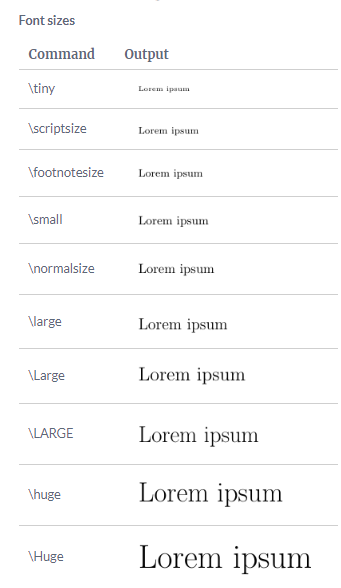
\includegraphics[scale=1]{../Font size.png} 

\section{Code Listing parameters}
Code listing parameters:\\
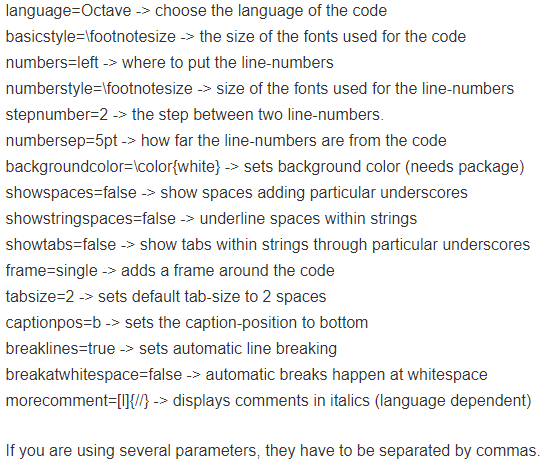
\includegraphics[scale=1]{../Code listing parameters.png} 

\section{Shadow frame in code listing}
Picture guide of shadow fraem in listing:\\
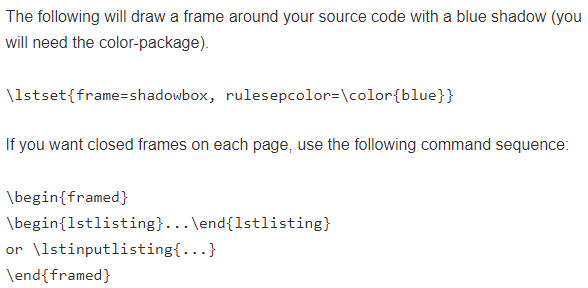
\includegraphics[scale=1]{../Shadow frame in code listing.png}

\section{Themes we can use in BEAMER class}
\subsection{Presentation themes without navigation bar}
\begin{enumerate}
 \item default
 \item boxes
 \item Bergen
 \item Boadilla
 \item Madrid
 \item AnnArbor
 \item CambridgeUS
 \item EastLansing
 \item Pittsburgh
 \item height=1 cm, Rochester
\end{enumerate}

\subsection{Presentation theme with a tree-like navigation bar}
\begin{enumerate}
 \item Antibes
 \item JuanLesPins
 \item Montpellier
 \item Berkeley
 \item Goettingen
 \item Marburg
 \item Hannover
 \item Berlin
 \item Ilmenau
 \item Dresden
 \item Darmstadt
 \item Frankfurt
 \item Singapore
 \item Szeged
\end{enumerate}

\section{\href{https://www.overleaf.com/learn/latex/List_of_Greek_letters_and_math_symbols}{List of Greek letters and math symbols}}
\begin{center}
	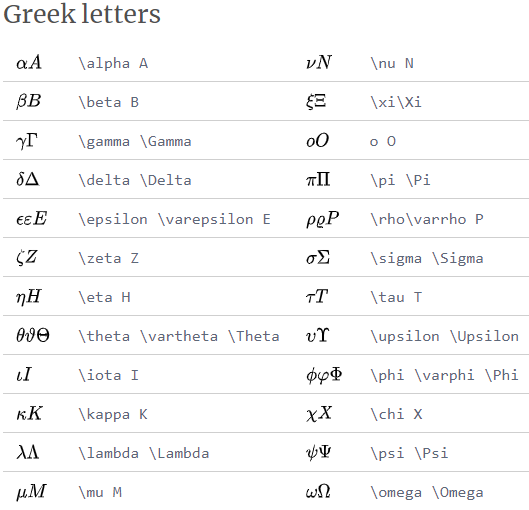
\includegraphics[width=200pt]{Greek Letters.png} 
	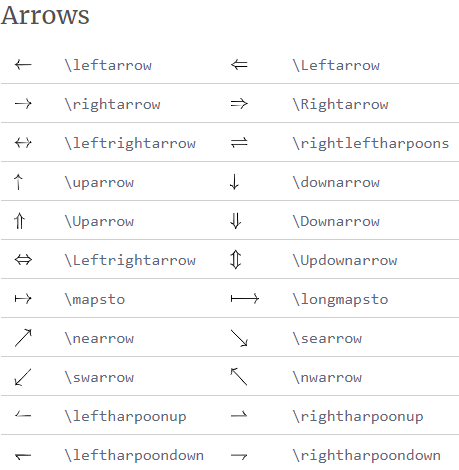
\includegraphics[width=200pt]{Arrows.png}
	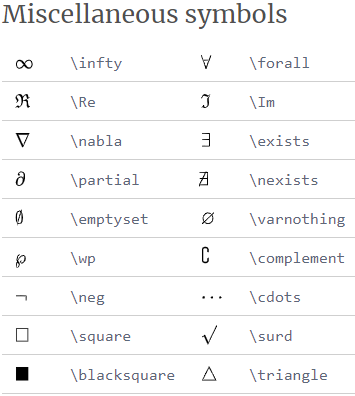
\includegraphics[width=200pt]{Miscellaneous symbols.png}
	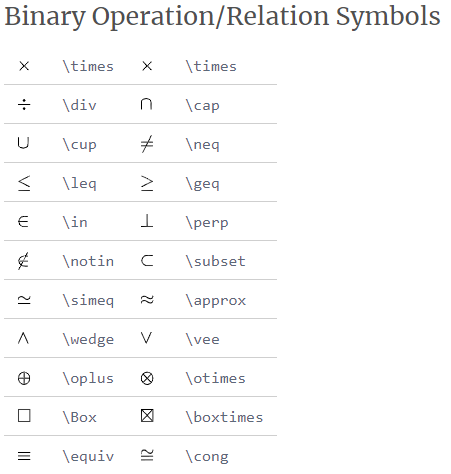
\includegraphics[width=200pt]{Binary Operation-Relation Symbols.png}
\end{center}

\section{Available Document Structure Commands}
\subsection{BOOK and REPORT}
\begin{itemize}
	\item part
	\item chapter
	\item section
	\item subsection
	\item subsubsection
	\item paragraph
	\item subparagraph
\end{itemize}

\subsection{ARTICLE}
\begin{itemize}
	\item part
	\item section
	\item subsection
	\item subsubsection
	\item paragraph
	\item subparagraph
\end{itemize}

\section{XeLaTeX}
\textcolor{blue}{XeLaTeX} is replacement for PDFLaTeX, it will takes input form LaTeX and turns output into a PDF. You cannot see instant created PDF file besides of TeXMaker.\linebreak
The major differences between \LaTeX{}/PDF\LaTeX{} are:

\begin{itemize}
	\item \textcolor{blue}{XeLaTeX} assumes input is in UTF-8(which allows encoding of non-English and non-Latin characters) by default.
	\item \textcolor{blue}{XeLaTeX} uses system fonts, not specially installed \LaTeX{} fonts.
\end{itemize}

It's packaged with TeXLive distribution of \LaTeX{}.

\section{The "hyperref" Package}
Include as \texttt{\textbackslash usepackage[hidelinks]{hyperref}}
For adding hyperlink / clickable link. \textit{hidelinks} will remove red frame form all type of links. While importing this package, it has to be the last package that are included. Because of, The \textit{hyperref} documentation says, "Make sure it comes last of your loaded packages". The reason is that it redefines many \LaTeX{} commands. It's a rule of thumb that helps you to avoid error. Also that, the \textit{amsrefs} user guide notes that, this package has to become after \textit{hyperref}.

\begin{center}
	\begin{tcolorbox}[enhanced,
		size=minimal, auto outer arc,
		width=2.1cm, octogon arc,
		colback=red, colframe=white, colupper=white,
		fontupper=\fontsize{7mm}{7mm}\selectfont\bfseries\sffamily,
		halign=center, valign=center,
		square,arc is angular,
		borderline={0.2mm}{-1mm}{blue!70!green}]
		OVER
	\end{tcolorbox}
\end{center}

\end{document}
